%The implementation of this project was created with the use of the \textit{JavaScript} open source libraries of \textit{React} and \textit{Redux}. 
%
The implementation of this project was developed as a web application. The \textit{front-end} or \textit{user interface} utilizes the \textit{JavaScript} open source library of \textit{React}. 
%
The \textit{back-end} was developed in \textit{JavaScript ES6}, and it utilizes the state management tool \textit{redux} to communicate with the \textit{front-end}. \\ \\
%
The web application mainly consists of four dependent \textit{React Components} named: \texttt{Data Manager}, \texttt{Fitting Manager}, \texttt{Learning Manager} and \texttt{Graph Matcher}. 
%
In this chapter we will explain how the components communicate between each other, and how they are used as routine to perform incremental analysis of system observations. 
%
%As \textit{React} projects are developed with the use of components, in this chapter we will discuss the main components (\textit{Data Manager}, \textit{Fitting Manager}, \textit{Learner}, \textit{Graph Matcher}) and data structures of the developed application for incremental learning.
%
%Use screenshots of the tool visual aid. 
%

\section{Data Manager}
As mentioned in \Cref{chap:incremental_Learning}, incremental learning begins by obtaining simulation data of an observed system. 
%
The \texttt{Data Manager}, which is the first section of our tool,  is in charge of organizing the data of simulations.
%
A simulation trace file from Uppaal can be imported and also visualized in the tool, as seen in the \textit{Data Plotted} from Figure \ref{data_manager}.
%
The information from the trace is parsed in this component as an \textit{array} of \textit{Map} objects that contain the points of the data per simulation run. 
%
The user can also pick the desired \textit{buffer size} and \textit{time step} value, which is going to be delivered to the \texttt{Fitting Manager}, along with the previous information for further analysis.
%
\begin{figure}[h]
	\centering
	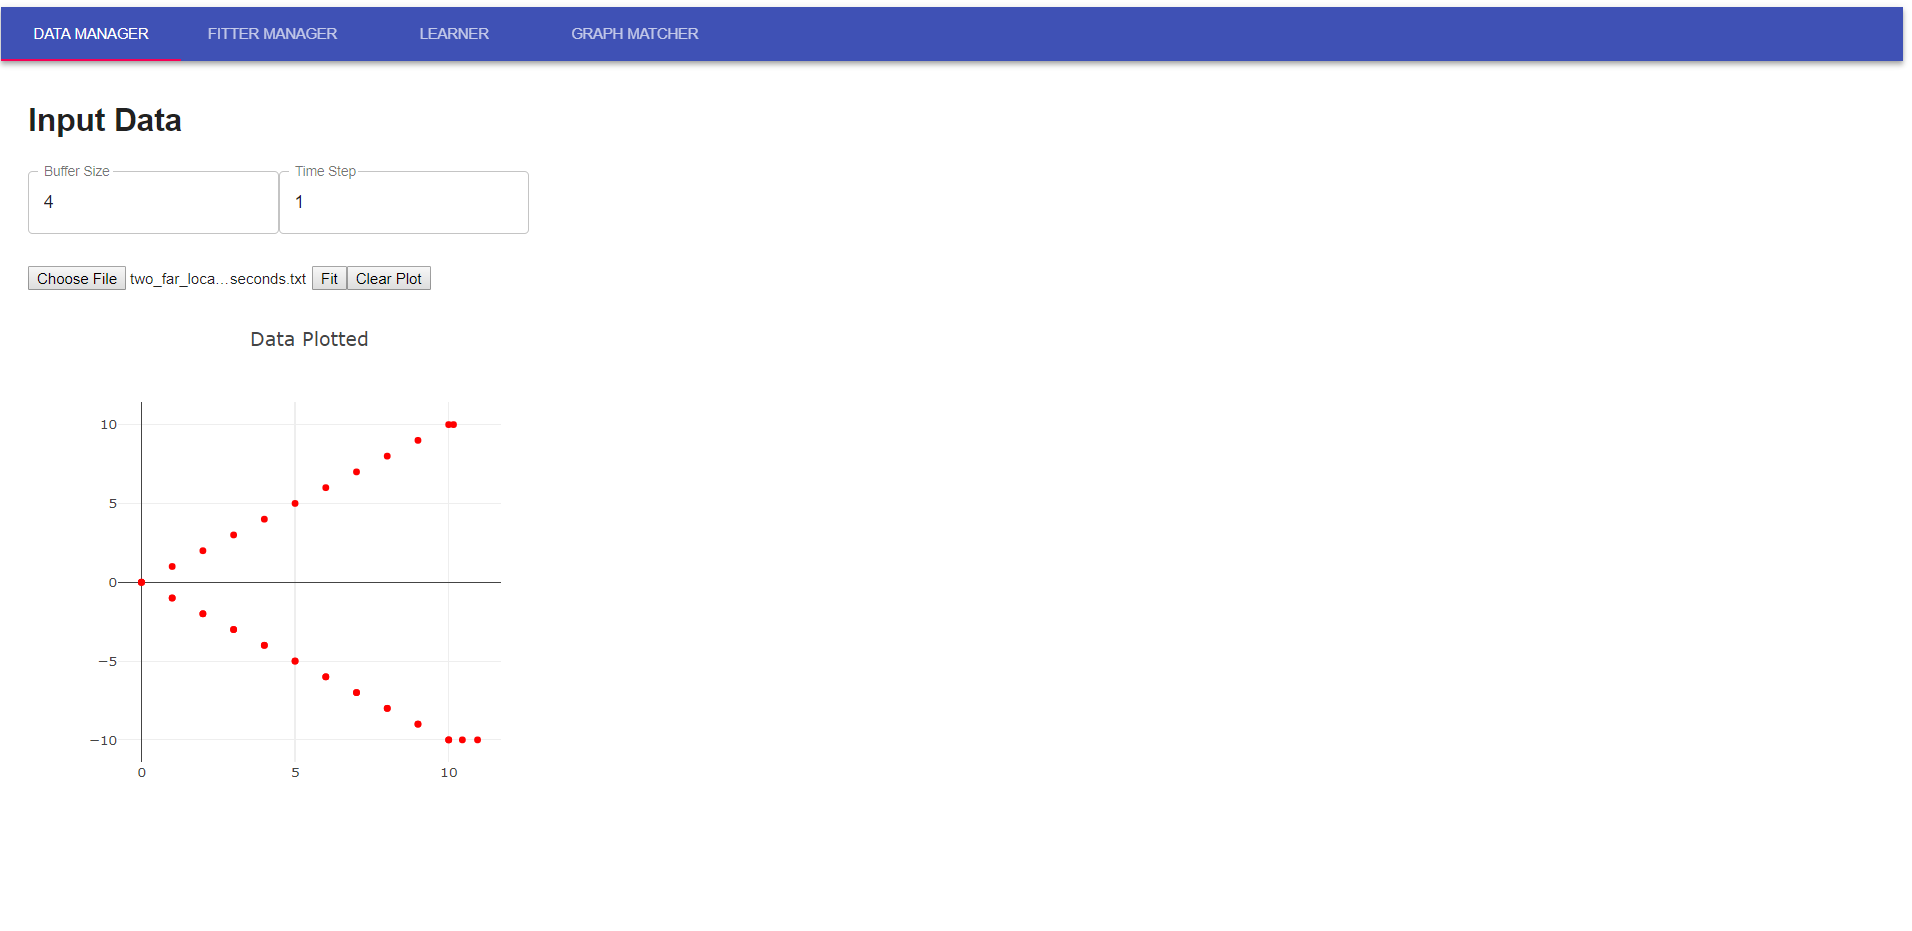
\includegraphics[scale=0.35]{./pictures/implementation/data_manager.png}
	\caption{Implementation Data Manager}
	\label{data_manager}
\end{figure}

\newpage

\section{Fitter Manager}
Given an array of maps created by the \texttt{Data Manager}, the \texttt{Fitter Manager} is in charge of fitting the observations from each map by utilizing Algorithm \ref{dataFitter} and the \textit{ml-levenberg-marquardt} library, to transform the array of maps into an array of \texttt{Equations} (structure shown in Figure \ref{equation_Structure}) which represent the behavior of an observed system, as seen in Figure \ref{fitter_manager} \\ \\
%
One can see in the \textit{Fitted Functions} text area, the results of fitting the information of each \textit{Simulation run}.
%
For every simulation run, there exists a section that contains the details of each fitted \texttt{Equation}. Let us take as an example the first fitted equation from \textit{Simulation 0}. The general information of the equation is written in black and contains the name of the equation (\textit{EQ1}), followed by the function structure ($ax+b$), the type of function that was fitted (\textit{linear}), and the \textit{Start-time} and \textit{End-Time}, that represent the range of time in which the observations were fitted. The details written in gray show the parameters that were fitted by the \textit{ml-levenberg-marquardt} library to evaluate the function, along with error of the calculations (\textit{Regression error}), that reflect the suitability of the fitted function with respect to the observed values.  
\begin{figure}[h]
	\centering
	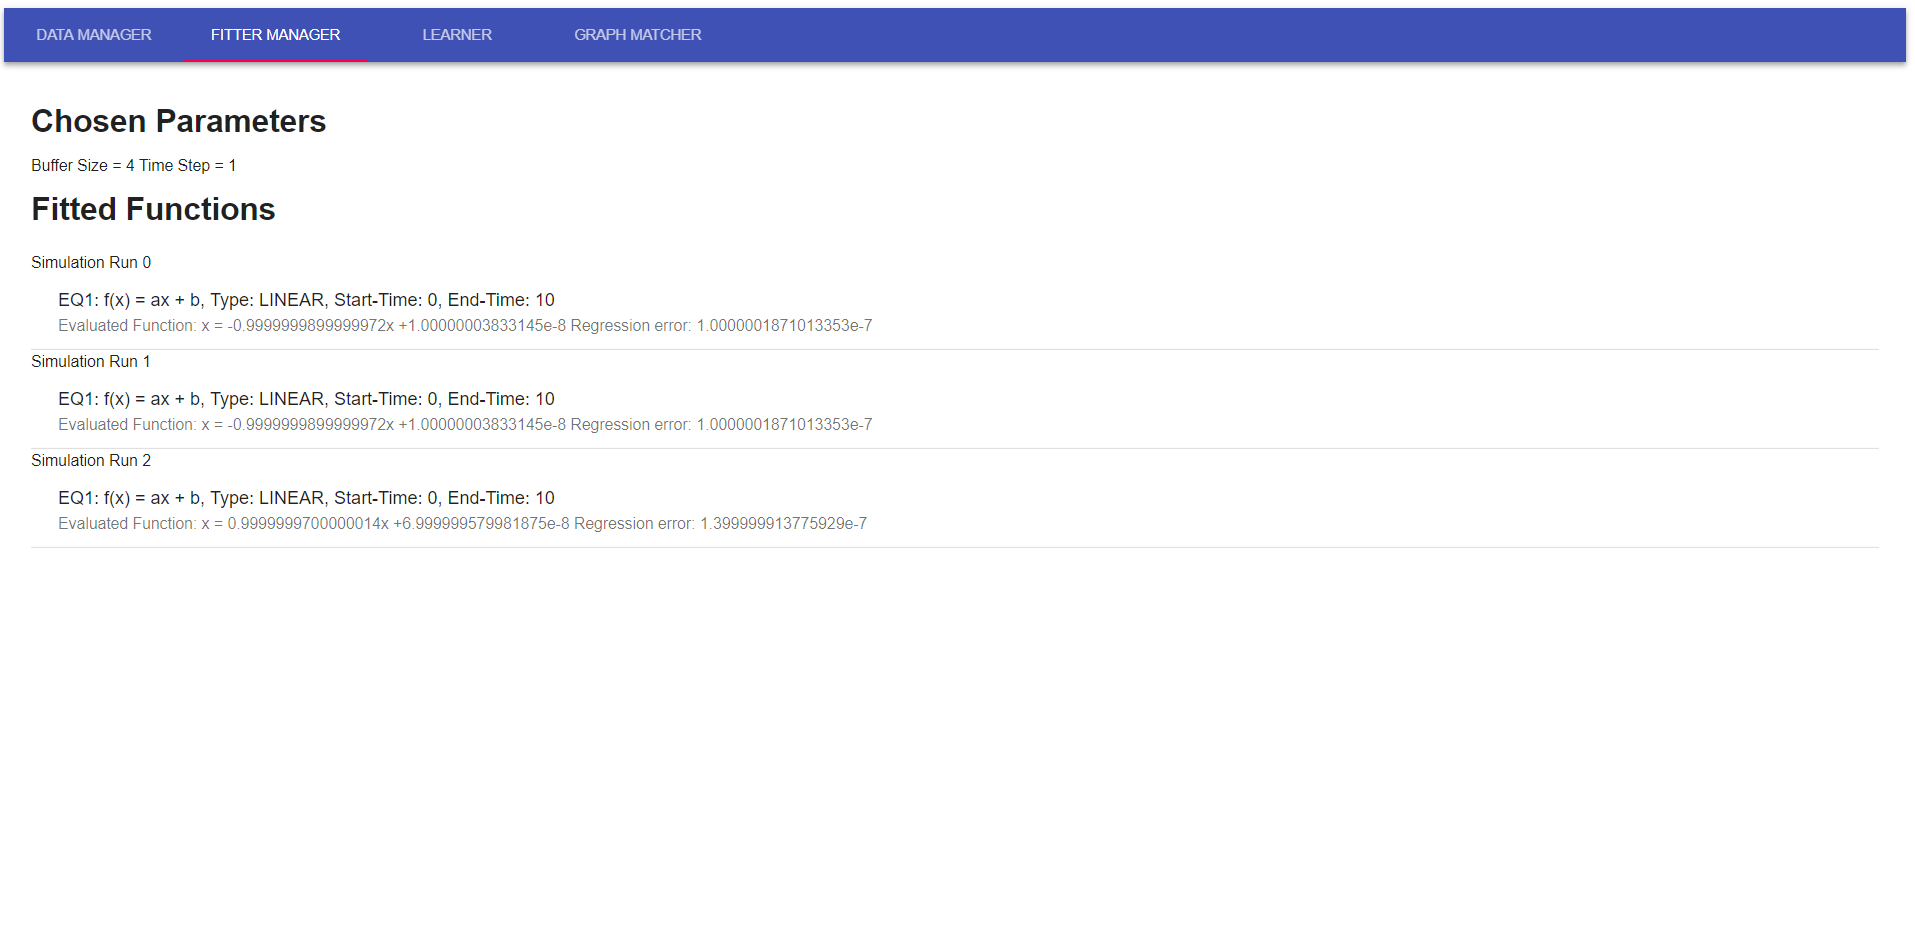
\includegraphics[scale=0.5]{./pictures/implementation/fitter_manager.png}
	\caption{Implementation Fitter Manager }
	\label{fitter_manager}
\end{figure}
\begin{figure}[t]
	\centering
	\begin{tikzpicture} 
	\umlclass{Equation}{ 
		id : string\\
		fittedFunction : string\\
		startTime : double\\
		endTime : double\\
	}{ } 
	\end{tikzpicture}
		\caption{Structure of an equation object}
	\label{equation_Structure}
\end{figure} 
 
\newpage
 
\section{Learning Manager}
%Explain in detail each cost evaluation and of how we decide to stop learning and jump to comparing or matching. 
The \texttt{Learning Manager} is responsible to perform the incremental learning approach, as explained in \Cref{chap:incremental_Learning}, with the values of the parameters that the user selects. By default, the \textit{Similarity Threshold} is set to 0.5, \textit{Time Cost} to 0.1, \textit{Functionality Cost} to 0.1 and \textit{Location Cost} to 0.5. Due to the fact that normalized Euclidean distance values between the range of zero and one are used in the incremental learning approach, we allowed to change the values of each parameter by this same range. One can also restrict the possible values of the parameters to a set of numbers (e.g. by choosing an option from the check-boxes) and learn observations for each possible combination.  
\\ \\
The tool begins the learning process after the user clicks the \textit{Learn} button. There exists two types of learning that the tool may perform: 1) With a model to reference, or 2) Without a model to reference. For the first approach, one can learn observations from systems but without evaluating the learning progress, as there is no possibility to interact with a model that resembles the observed system. Whereas in the second approach, one can import a model that resembles the observed system (e.g. Original model) producing the observations, so that the similarity of the models can also be measured \textit{on-the-fly}. Nevertheless, it is possible for both types of learning to visualize the evolution of the learned model, by selecting the desired model from the \textit{Learned Models} drop-down list. It is also important to notice that the models are constructed as directed acyclic graphs, with the only exception that \textit{self-loops} are allowed, as seen in in Figure \ref{learning_manager}. 
%
\begin{figure}[h]
	\centering
	\makebox[\textwidth][c]{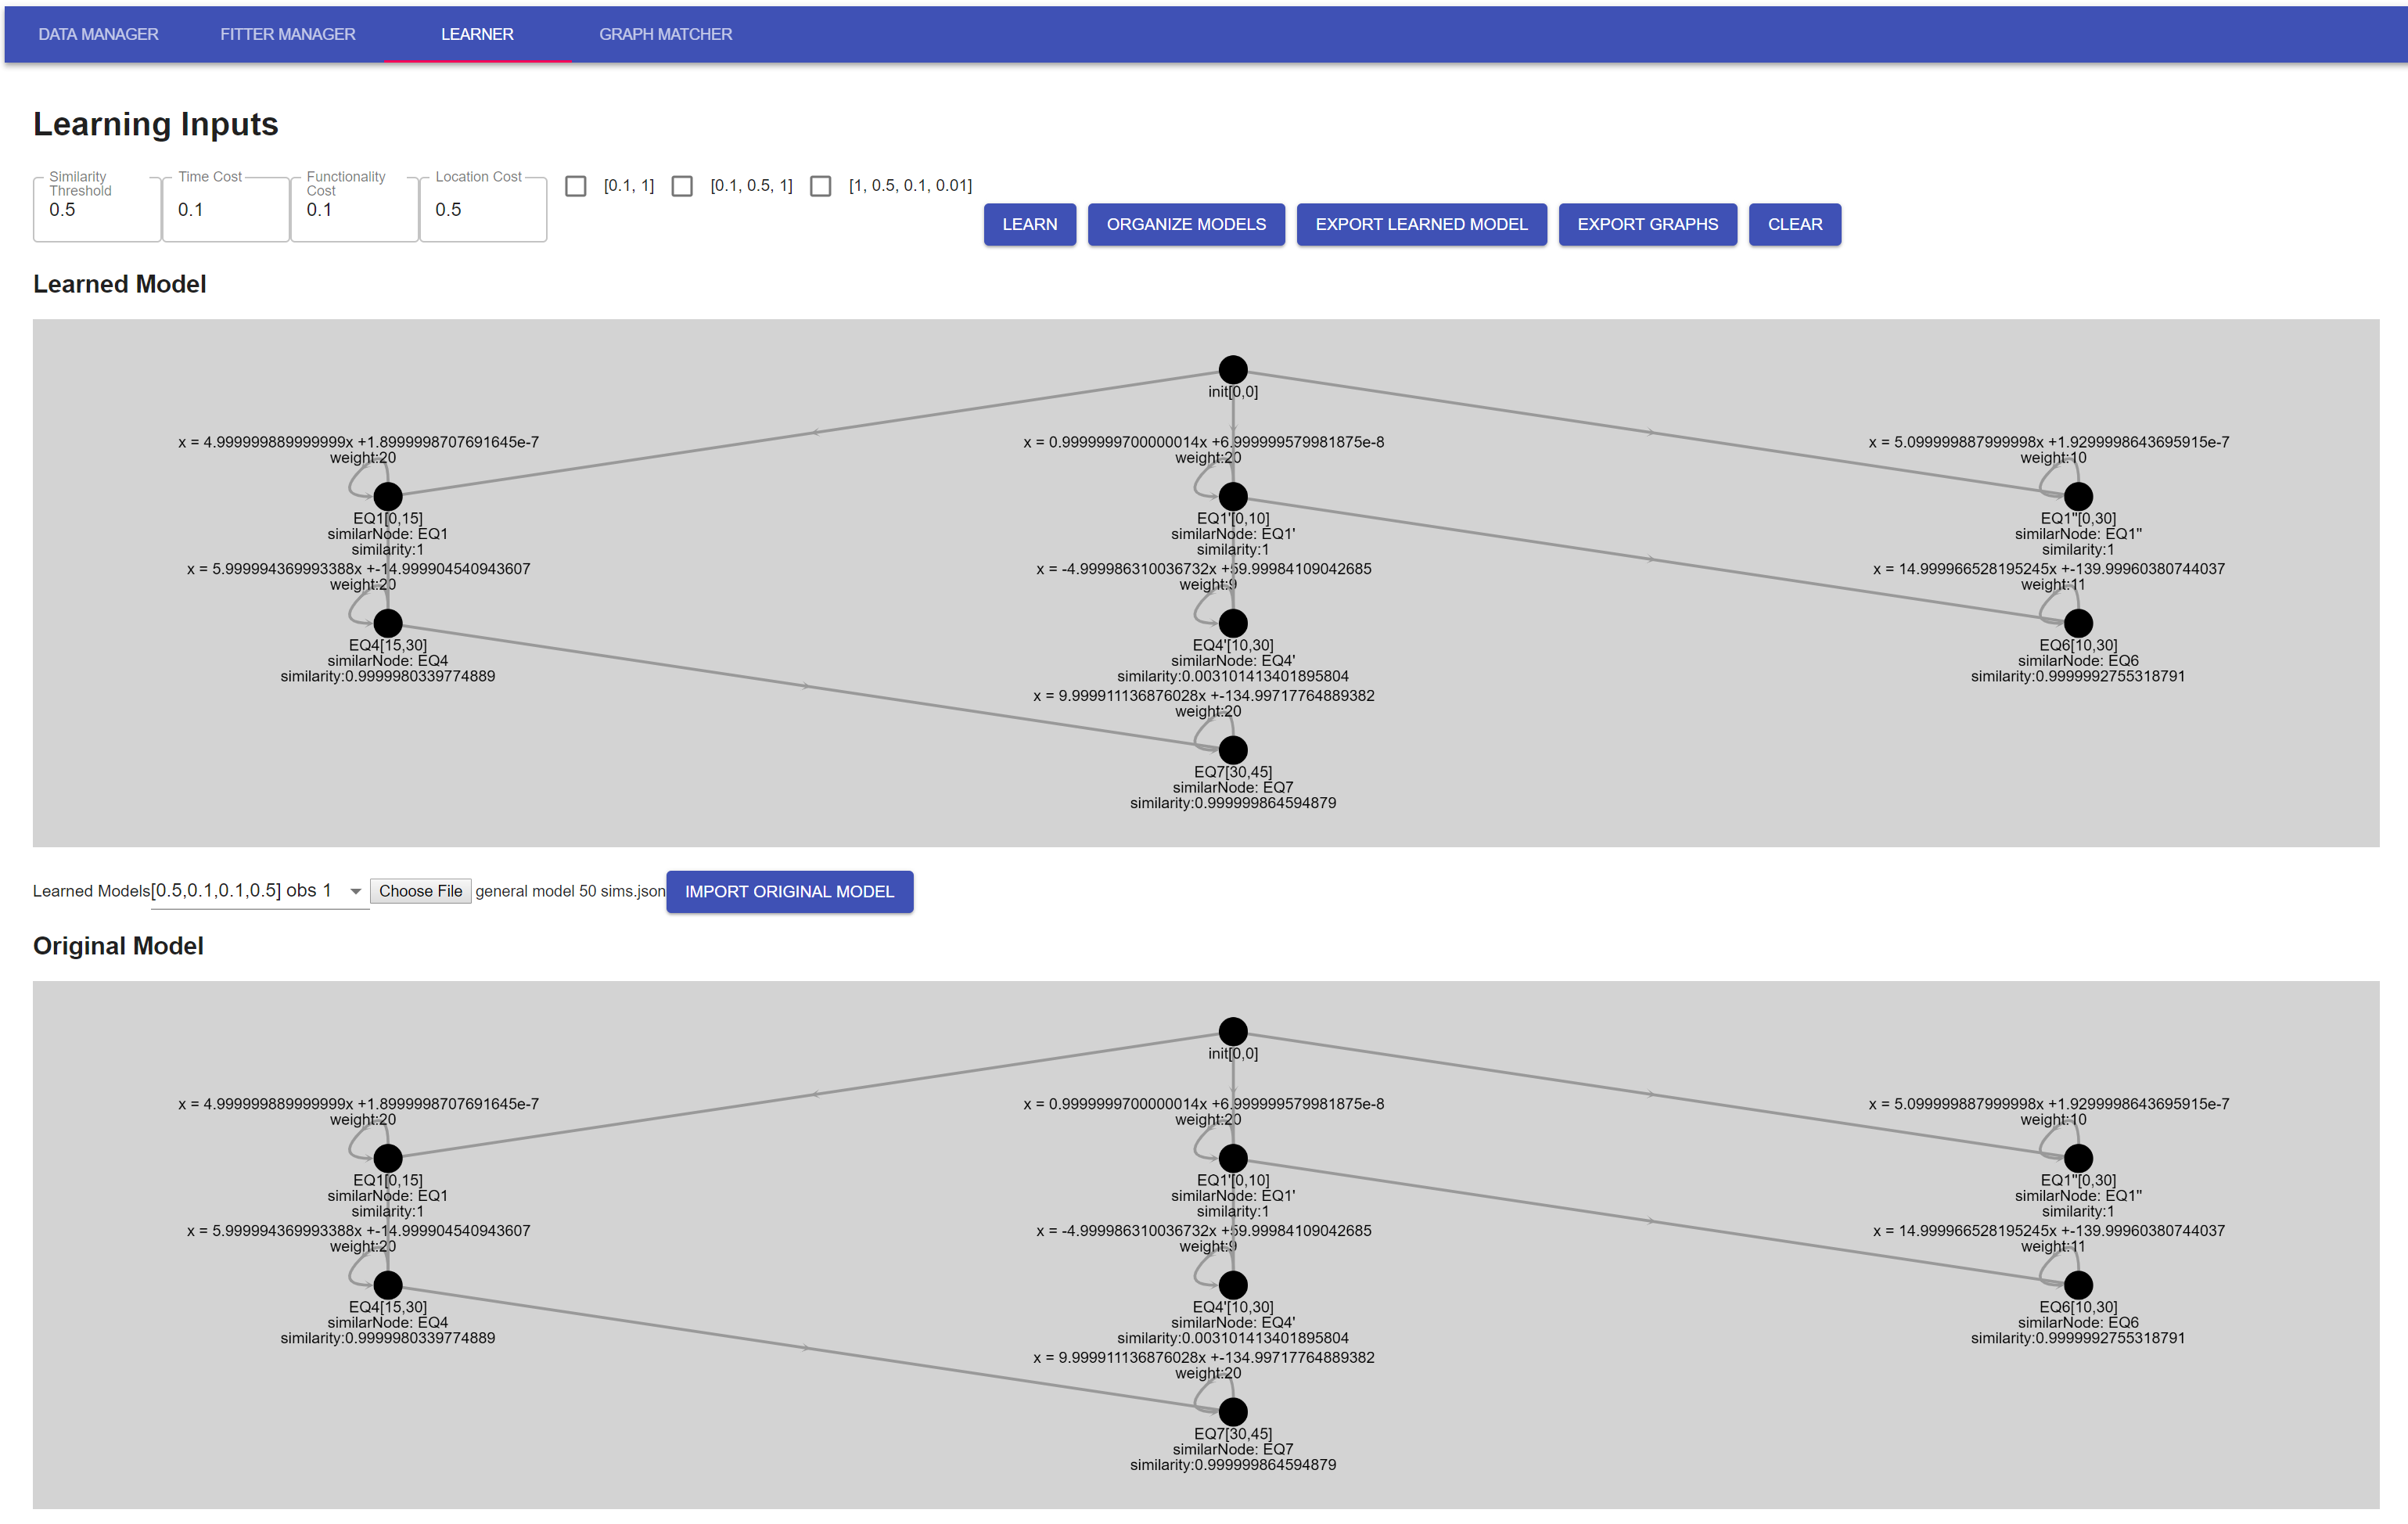
\includegraphics[width=1.1\textwidth]{./pictures/implementation/learning_manager.png}}%
%	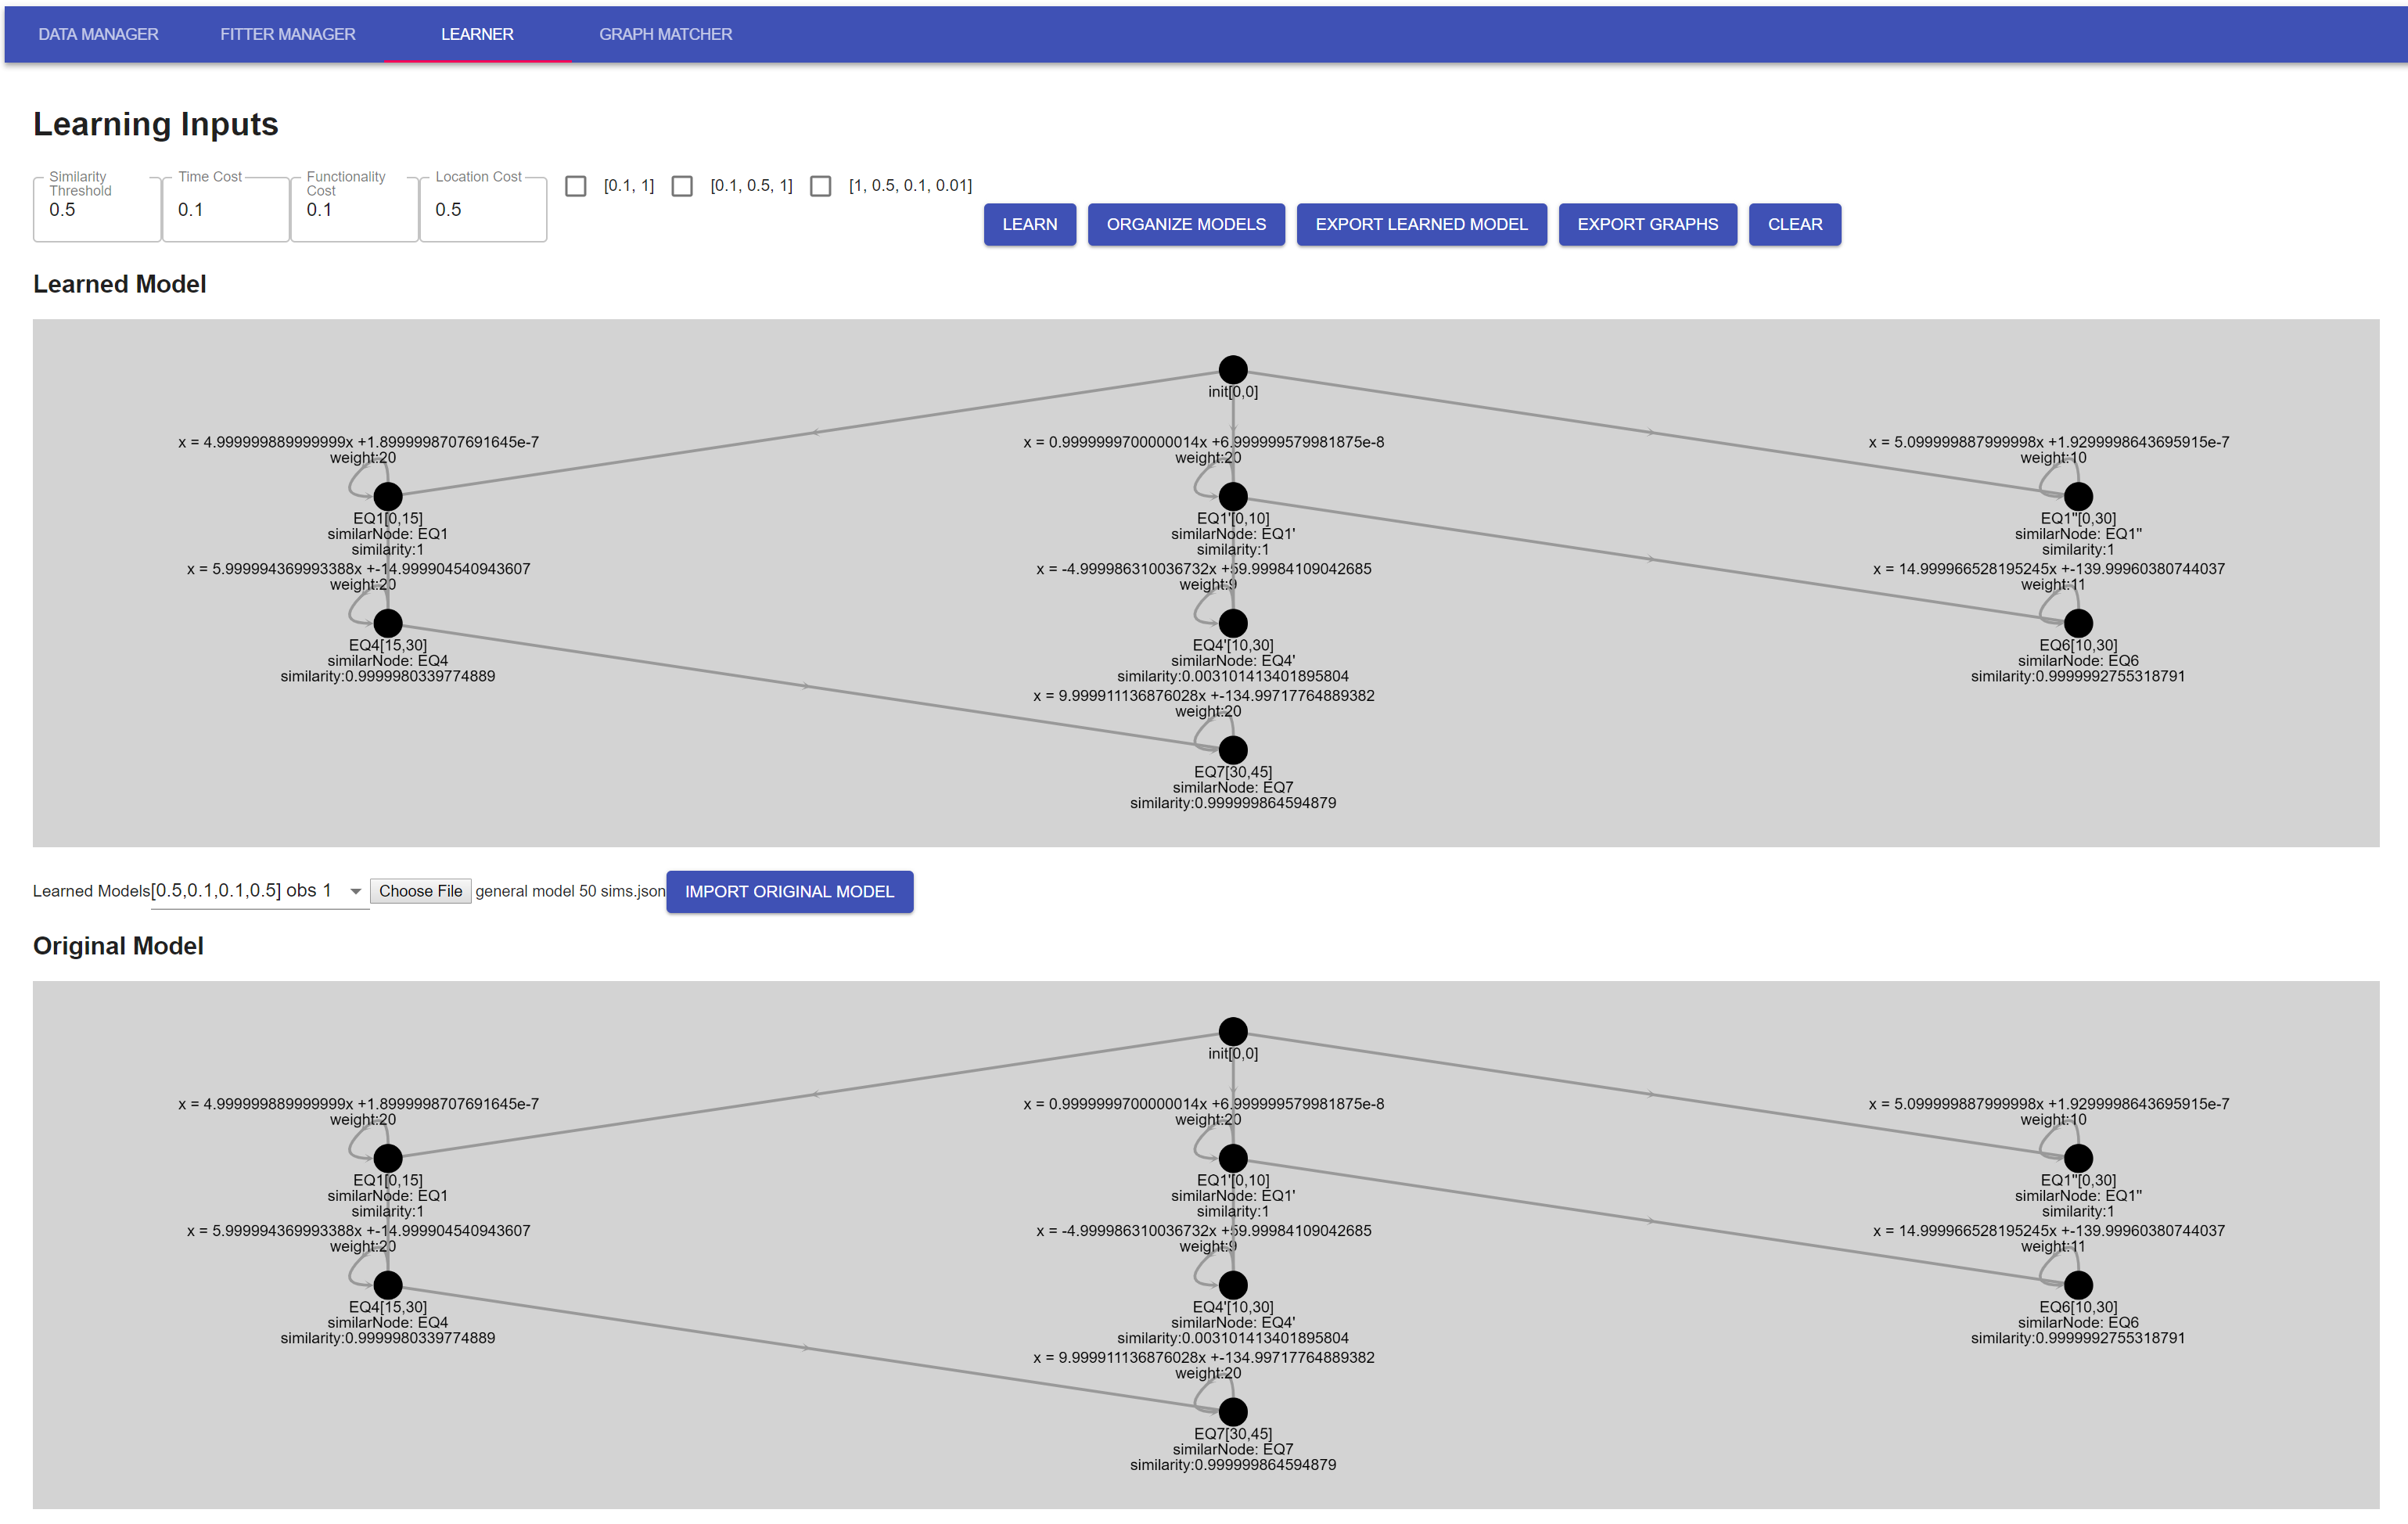
\includegraphics[scale=0.25]{./pictures/implementation/learning_manager.png}
	\caption{Implementation Learning Manager}
	\label{learning_manager}
\end{figure}

\newpage

\section{Graph Matcher}
The \texttt{Graph Matcher} component was created for visualizing how the matching of models is performed in incremental learning, whenever there exists an \textit{original model} (e.g. the imported model from \texttt{Learning Manager}) that can be compared against the \textit{learned model}. 
%
The similarity of the models is calculated by traversing both graphs simultaneously and matching the nodes, disregarding their labels and only by judging how close they are in terms of Euclidean distance. The user interface of the \texttt{Graph Matcher}, as seen in Figure \ref{graph_matcher} is essentially the same as the one from the \texttt{Learning Manager}, with an additional section called \textit{Matched Model}, where one can see which nodes from the learned model were matched with the ones from the original model. For simplicity and explanation purposes, we matched the two models from Figure \ref{learning_manager} and show the results in Figure \ref{graph_matcher_matched}. As seen in Figure \ref{graph_matcher_matched}, the learned model was successfully matched, as it is identical to the original model. The \textit{Graph Matcher} facilitates the interpretation of the comparison by coloring the edges and nodes in green when they were matched, and in red when they were not. Also, the \textit{Matched Model} section includes information of which node from the learned model was matched in the original model. The label \textit{lm} represents the name of the node of the learned model, and the label \textit{om} corresponds to the name of the node from the original model that was matched.
%
\begin{figure}[h]
	\centering
	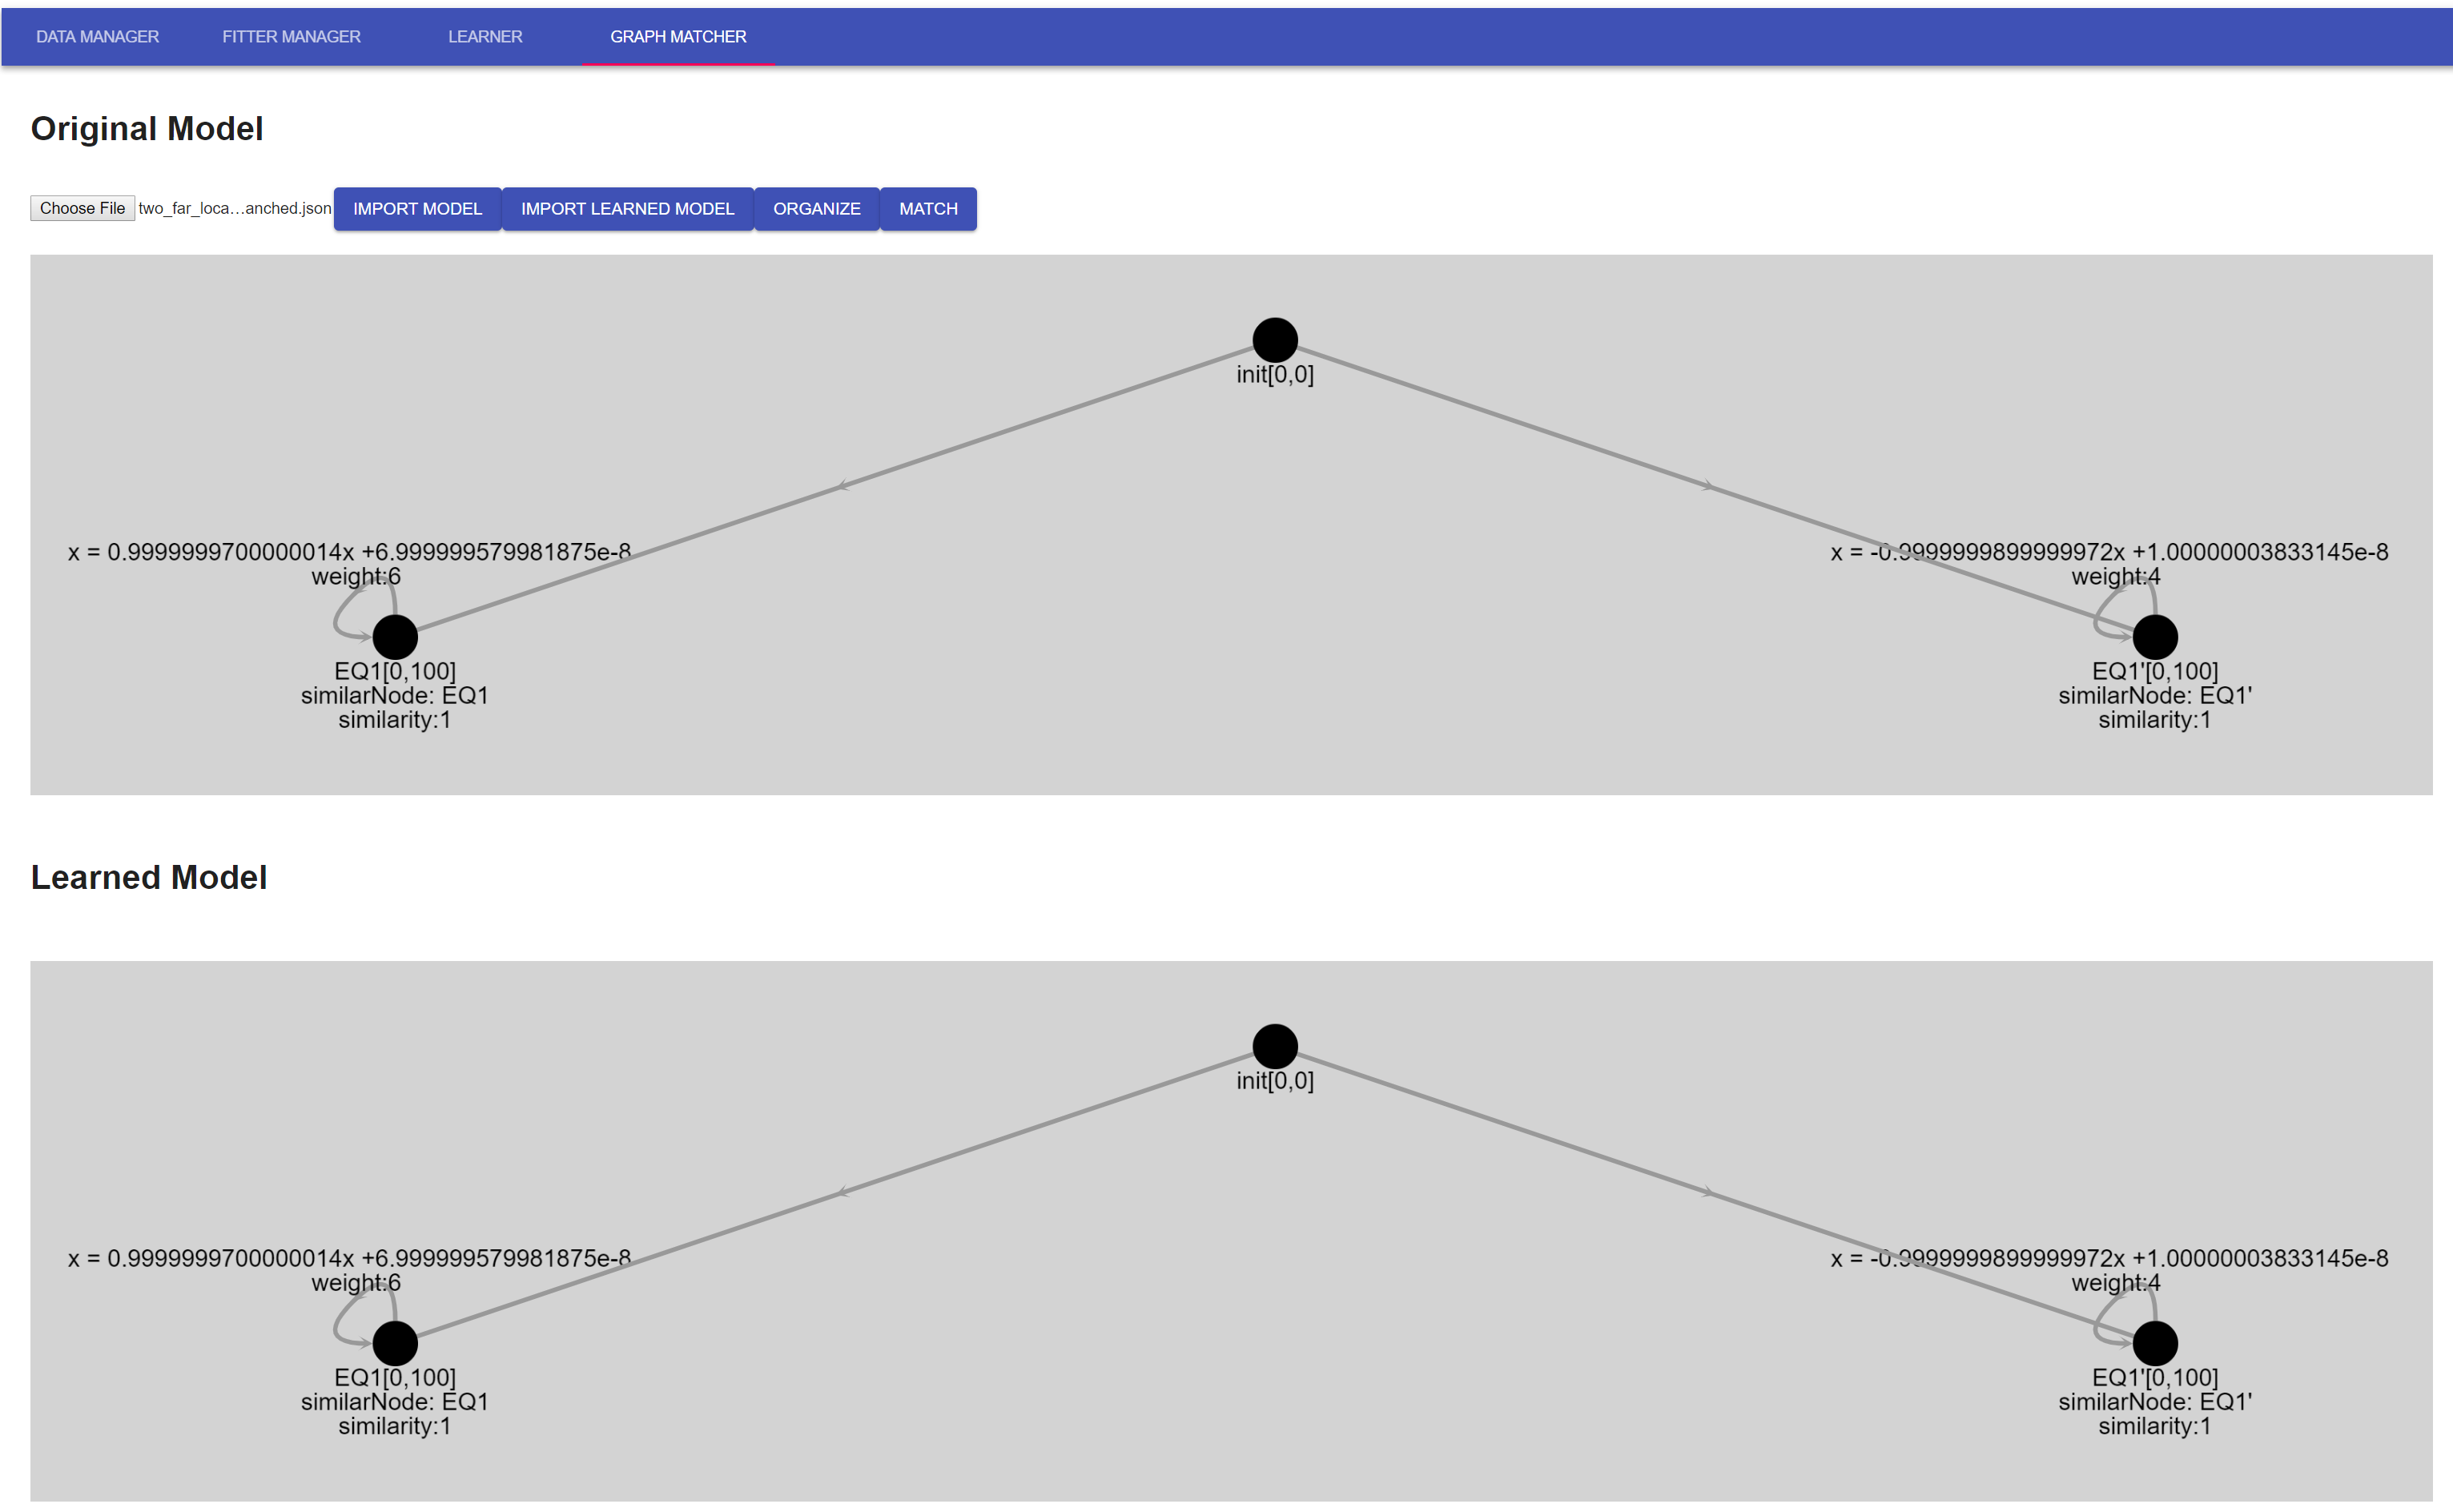
\includegraphics[scale=0.25]{./pictures/implementation/Graph_Matcher.png}
	\caption{Implementation Graph Matcher}
	\label{graph_matcher}
\end{figure}
\begin{figure}[h]
	\centering
	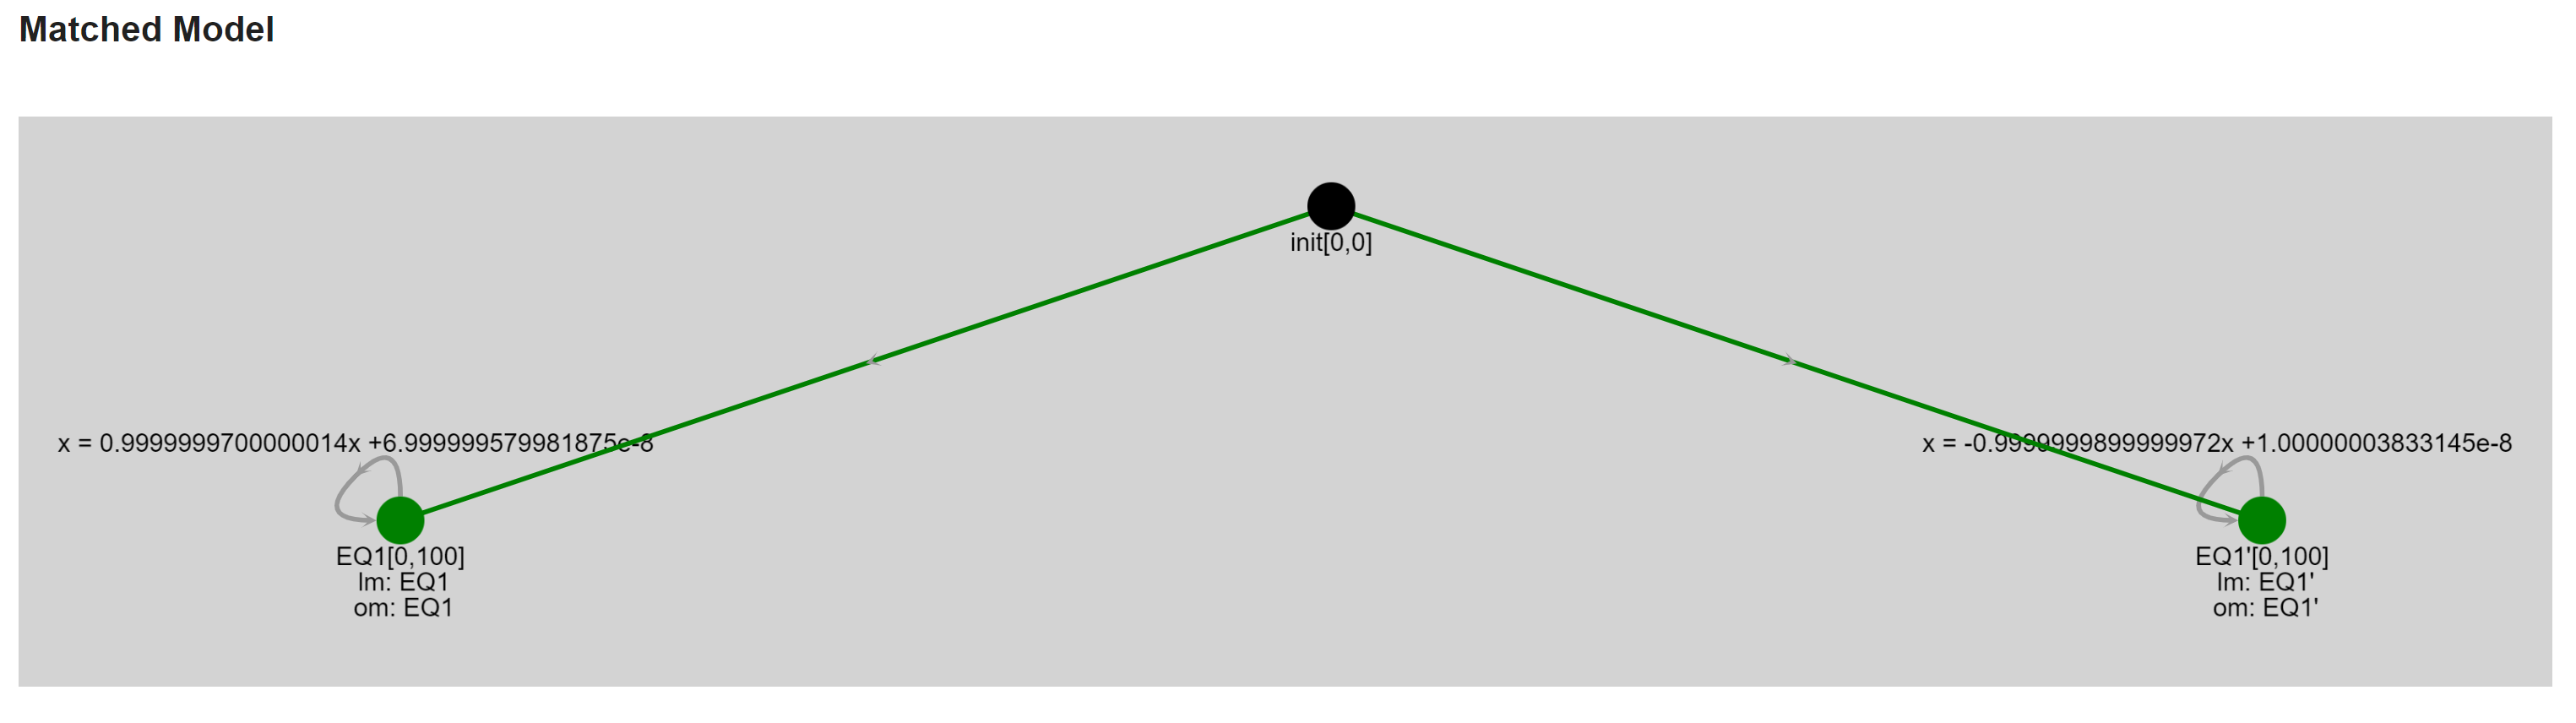
\includegraphics[scale=0.25]{./pictures/implementation/Graph_Matcher_1.png}
	\caption{Implementation Graph Matcher - Model matched section}
	\label{graph_matcher_matched}
\end{figure}




